\documentclass[12pt,a4paper]{article}

\usepackage[margin=24mm]{geometry}
\usepackage{fontspec}
\usepackage{xeCJK}
\usepackage{graphicx}
\usepackage{booktabs}
\usepackage{float}
\usepackage{amsmath}
\usepackage{array}
\usepackage{caption}
\usepackage{hyperref}
\usepackage{tikz}
\usetikzlibrary{arrows.meta}

\setmainfont{Microsoft JhengHei}
\setCJKmainfont{Microsoft JhengHei}
\graphicspath{{./}}
\sloppy

\title{Bui Table 1/2 屈曲算例重現}
\author{}
\date{}

\begin{document}
\maketitle

\section{本文使用的屈曲公式}
Mindlin 板位移場為
\[
\bar{u}_{\alpha}(x_1,x_2,x_3)
=u_{\alpha}(x_1,x_2)-x_3\phi_{\alpha},
\qquad
\bar{u}_3=w .
\]
應變、曲率與剪切應變為
\[
\epsilon_{\alpha\beta}
=\varepsilon_{\alpha\beta}+x_3\kappa_{\alpha\beta},
\qquad
\varepsilon_{\alpha\beta}
=\frac{1}{2}(u_{\alpha,\beta}+u_{\beta,\alpha}),
\]
\[
\kappa_{\alpha\beta}
=-\frac{1}{2}(\phi_{\alpha,\beta}+\phi_{\beta,\alpha}),
\qquad
\gamma_\alpha=2\epsilon_{\alpha3}=w_{,\alpha}-\phi_\alpha .
\]

材料關係與厚度積分後的合力為
\[
\sigma_{\alpha\beta}
=D_{\alpha\beta\gamma\eta}\epsilon_{\gamma\eta},
\qquad
\tau_{3\alpha}=G\gamma_\alpha ,
\]
\[
D_{\alpha\beta\gamma\eta}
=\frac{E}{1-\nu^2}\left[
\nu\delta_{\alpha\beta}\delta_{\gamma\eta}
+\frac{1-\nu}{2}
(\delta_{\alpha\gamma}\delta_{\beta\eta}
+\delta_{\alpha\eta}\delta_{\beta\gamma})
\right],
\qquad
G=\frac{E}{2(1+\nu)},
\]
\[
M_{\alpha\beta}
=\int_{-h/2}^{h/2}x_3\sigma_{\alpha\beta}\,dx_3
=\frac{h^3}{12}D_{\alpha\beta\gamma\eta}\kappa_{\gamma\eta},
\qquad
Q_\alpha=k_sGh\,\gamma_\alpha .
\]

考慮初始面內力 \(P_{\alpha\beta}\) 的幾何效應，弱式為
\[
\int_{\Omega}
\left(
M_{\alpha\beta}\delta\kappa_{\alpha\beta}
+Q_\alpha\delta\gamma_\alpha
-P_{\alpha\beta}w_{,\alpha}\delta w_{,\beta}
\right)d\Omega=0 .
\]
也就是
\[
a_b(\boldsymbol\phi,\delta\boldsymbol\phi)
+a_s((w,\boldsymbol\phi),(\delta w,\delta\boldsymbol\phi))
-a_g(w,\delta w)=0 .
\]

形函數離散採
\[
w^h=\sum_KN_Kw_K,\qquad
\phi_x^h=\sum_RN_R\phi_{xR},\qquad
\phi_y^h=\sum_RN_R\phi_{yR}.
\]


彎曲剛度只作用在轉角自由度：
\[
a_b(\boldsymbol\phi,\delta\boldsymbol\phi)
=\int_{\Omega}\frac{h^3}{12}
D_{\alpha\beta\gamma\eta}
\kappa_{\alpha\beta}\delta\kappa_{\gamma\eta}\,d\Omega
=\sum_{R,S}\delta\phi_{iR}
\left(K_{\phi\phi,RS}^b\right)_{ij}\phi_{jS}.
\]
其子矩陣為
\[
\begin{aligned}
\left(K_{\phi\phi,RS}^b\right)_{11}
&=\frac{h^3}{12}\int_{\Omega}
\left(D_{1111}N_{R,x}N_{S,x}
+D_{1212}N_{R,y}N_{S,y}\right)d\Omega,\\
\left(K_{\phi\phi,RS}^b\right)_{12}
&=\frac{h^3}{12}\int_{\Omega}
\left(D_{1122}N_{R,x}N_{S,y}
+D_{1212}N_{R,y}N_{S,x}\right)d\Omega,\\
\left(K_{\phi\phi,RS}^b\right)_{21}
&=\frac{h^3}{12}\int_{\Omega}
\left(D_{1122}N_{R,y}N_{S,x}
+D_{1212}N_{R,x}N_{S,y}\right)d\Omega,\\
\left(K_{\phi\phi,RS}^b\right)_{22}
&=\frac{h^3}{12}\int_{\Omega}
\left(D_{1212}N_{R,x}N_{S,x}
+D_{1111}N_{R,y}N_{S,y}\right)d\Omega .
\end{aligned}
\]

剪切剛度由
\[
a_s((w,\boldsymbol\phi),(\delta w,\delta\boldsymbol\phi))
=\int_\Omega k_sGh\,\gamma_\alpha\delta\gamma_\alpha\,d\Omega
\]
展開成四個區塊：
\[
K_{ww,KL}^s
=k_sGh\int_{\Omega}
\left(N_{K,x}N_{L,x}+N_{K,y}N_{L,y}\right)d\Omega,
\]
\[
K_{\phi\phi,KL}^s
=k_sGh\int_{\Omega}N_KN_L\,d\Omega\,I_2,
\]
\[
\left(K_{w\phi,KL}^s\right)_1
=-k_sGh\int_{\Omega}N_{K,x}N_L\,d\Omega,
\qquad
\left(K_{w\phi,KL}^s\right)_2
=-k_sGh\int_{\Omega}N_{K,y}N_L\,d\Omega,
\]
\[
\left(K_{\phi w,KL}^s\right)_1
=-k_sGh\int_{\Omega}N_KN_{L,x}\,d\Omega,
\qquad
\left(K_{\phi w,KL}^s\right)_2
=-k_sGh\int_{\Omega}N_KN_{L,y}\,d\Omega .
\]

幾何剛度只作用於 \(w\) 區塊：
\[
a_g(w,\delta w)
=P_{\alpha\beta}\int_{\Omega}
w_{,\alpha}\delta w_{,\beta}\,d\Omega,
\qquad
K_{ww,KL}^g
=P_{\alpha\beta}\int_{\Omega}
N_{K,\alpha}N_{L,\beta}\,d\Omega .
\]

因此整體分塊矩陣為
\[
\begin{bmatrix}
K_{ww}^{s} & K_{w\phi}^{s} \\
K_{\phi w}^{s} & K_{\phi\phi}^{b}+K_{\phi\phi}^{s}
\end{bmatrix}
\begin{bmatrix}
d_w\\ d_{\phi}
\end{bmatrix}
-
\begin{bmatrix}
K_{ww}^{g} & 0\\
0 & 0
\end{bmatrix}
\begin{bmatrix}
d_w\\ d_{\phi}
\end{bmatrix}
=0 .
\]

屈曲特徵值計算寫為
\[
K\boldsymbol d=\lambda K_g\boldsymbol d,
\qquad
K=K^b+K^s .
\]
Table 1/2 的單軸壓縮使用
\[
P_{11}=1,\qquad P_{22}=0,\qquad P_{12}=0,
\]
最後轉成無因次屈曲係數
\[
k=\frac{\lambda_{cr}b^2}{\pi^2D},
\qquad
D=\frac{Eh^3}{12(1-\nu^2)}.
\]
若參考面內合力取 \(P_{\alpha\beta}^{ref}=1\)，則特徵值本身對應臨界面內合力 \(N_{cr}=\lambda_{cr}\)。因此單軸壓縮的臨界應力可由
\[
\sigma_{cr}=\frac{N_{cr}}{h}
=\frac{\lambda_{cr}}{h}
=k\frac{\pi^2D}{b^2h}
\]
換算；純剪算例則同理記為
\[
\tau_{cr}=\frac{\lambda_{cr}}{h}.
\]

\section{Table 1：邊界與節點密度}

這組資料用來檢查單軸壓縮方板在不同邊界條件與節點密度下的收斂情形。條件為 \(a/b=1\)、\(h/b=0.01\)、\(E=200\times10^9\)、\(\nu=0.3\)、\(k_s=5/6\)，載重為 \(P_{11}=1\)、\(P_{22}=P_{12}=0\)，節點配置由 \(7\times7\) 增加到 \(17\times17\)。

\begin{figure}[H]
    \centering
    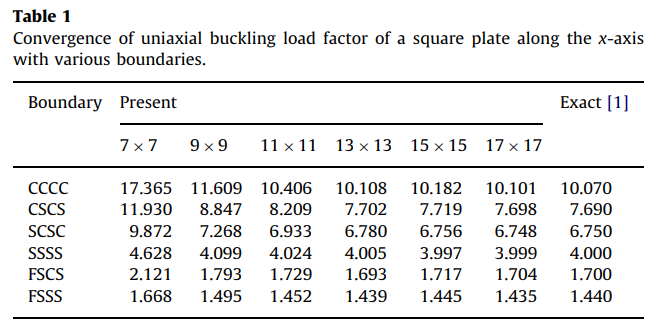
\includegraphics[width=\textwidth]{table1.png}
    \caption{Table 1 原始截圖。}
\end{figure}

下表採用相同測試規格，Present 數值由本文公式重新計算；Exact [1] 保留作為參考。

\begin{table}[H]
\centering
\caption{Table 1 規格重新計算結果}
\resizebox{\textwidth}{!}{%
\begin{tabular}{cccccccc}
\toprule
Boundary & 7x7 & 9x9 & 11x11 & 13x13 & 15x15 & 17x17 & Exact [1] \\
\midrule
CCCC & 951.2794 & 536.2115 & 346.6046 & 244.1826 & 182.5804 & 142.6401 & 10.07 \\
CSCS & 684.8616 & 397.6406 & 260.9281 & 185.4208 & 139.3923 & 109.285 & 7.69 \\
SCSC & 620.2962 & 350.169 & 226.9719 & 160.2938 & 120.0986 & 93.9836 & 6.75 \\
SSSS & 377.7068 & 225.6285 & 150.5352 & 108.1273 & 81.8756 & 64.5065 & 4 \\
FSCS & 178.7335 & 102.9857 & 67.2599 & 47.6294 & 35.7002 & 27.9128 & 1.7 \\
FSSS & 141.8823 & 82.3535 & 54.0382 & 38.3929 & 28.8474 & 22.5972 & 1.44 \\
\bottomrule
\end{tabular}%
}
\end{table}

由於 Table 1 的主表已經很寬，下面另列由 Present \(k\) 換算出的 Present \(\sigma_{cr}\)。本組算例使用 \(E=200\times10^9\)、\(h/b=0.01\)、\(b=1\)，因此 \(\sigma_{cr}\) 以 MPa 表示。

\begin{table}[H]
\centering
\caption{Table 1 臨界應力 \(\sigma_{cr}\)（MPa）}
\resizebox{\textwidth}{!}{%
\begin{tabular}{cccccccc}
\toprule
Boundary & 7x7 & 9x9 & 11x11 & 13x13 & 15x15 & 17x17 & Exact [1] \\
\midrule
CCCC & 17195.52 & 9692.67 & 6265.29 & 4413.89 & 3300.36 & 2578.39 & 182.03 \\
CSCS & 12379.69 & 7187.83 & 4716.59 & 3351.70 & 2519.68 & 1975.46 & 139.01 \\
SCSC & 11212.60 & 6329.72 & 4102.79 & 2897.50 & 2170.93 & 1698.87 & 122.01 \\
SSSS & 6827.50 & 4078.51 & 2721.10 & 1954.53 & 1480.00 & 1166.03 & 72.30 \\
FSCS & 3230.82 & 1861.59 & 1215.80 & 860.96 & 645.32 & 504.56 & 30.73 \\
FSSS & 2564.69 & 1488.64 & 976.81 & 694.00 & 521.45 & 408.47 & 26.03 \\
\bottomrule
\end{tabular}%
}
\end{table}

\section{Table 2：文獻方法比較}

這組資料用來把本文 Present 結果放進原表的比較欄位中。條件為 \(a/b=1\)、\(h/b=0.01\)、\(E=200\times10^9\)、\(\nu=0.3\)、\(k_s=5/6\)，載重同樣為 \(P_{11}=1\)、\(P_{22}=P_{12}=0\)，Present 固定使用 \(13\times13\) 節點結果。

\begin{figure}[H]
    \centering
    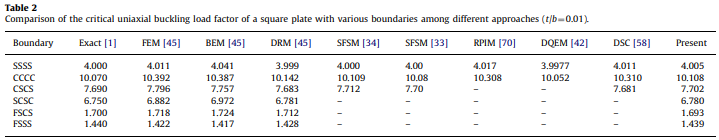
\includegraphics[width=\textwidth]{table2.png}
    \caption{Table 2 原始截圖。}
\end{figure}

下表保留原表的參考方法欄位，只有 Present 欄位改由本文公式重新計算；空白表示原表未提供該數值。

\begin{table}[H]
\centering
\caption{Table 2 規格重新計算與參考方法比較}
\resizebox{\textwidth}{!}{%
\begin{tabular}{ccccccccccccc}
\toprule
Boundary & Exact [1] & Exact \(\sigma_{cr}\) (MPa) & FEM [45] & BEM [45] & DRM [45] & SFSM [34] & SFSM [33] & RPIM [70] & DQEM [42] & DSC [58] & Present \(k\) & Present \(\sigma_{cr}\) (MPa) \\
\midrule
CCCC & 10.07 & 182.03 & 10.392 & 10.387 & 10.142 & 10.109 & 10.08 & 10.308 & 10.052 & 10.31 & 244.1826 & 4413.89 \\
CSCS & 7.69 & 139.01 & 7.796 & 7.757 & 7.683 & 7.712 & 7.7 &  &  & 7.681 & 185.4208 & 3351.70 \\
SCSC & 6.75 & 122.01 & 6.882 & 6.972 & 6.781 &  &  &  &  &  & 160.2938 & 2897.50 \\
SSSS & 4 & 72.30 & 4.011 & 4.041 & 3.999 & 4 & 4 & 4.017 & 3.9977 & 4.011 & 108.1273 & 1954.53 \\
FSCS & 1.7 & 30.73 & 1.718 & 1.724 & 1.712 &  &  &  &  &  & 47.6294 & 860.96 \\
FSSS & 1.44 & 26.03 & 1.422 & 1.417 & 1.428 &  &  &  &  &  & 38.3929 & 694.00 \\
\bottomrule
\end{tabular}%
}
\end{table}

\section{補充算例}

以下四組資料用來檢查同一套 \(K^b,K^s,K^g\) 組裝方式在不同幾何比例與載重組合下的反應。這些表格保留 Reference/Exact、Present 與誤差欄位，方便直接核對目前公式的尺度差異。

\subsection{單軸壓縮矩形板}

此表改變 \(a/b\)，邊界為 SSSS，載重為單軸壓縮。它用來檢查幾何長寬比改變時，屈曲係數是否呈現合理趨勢。材料與厚度設定為 \(E=30\times10^6\) psi、\(\nu=0.3\)、\(k_s=5/6\)、\(h/b=0.01\)，載重為 \(P_{11}=1\)、\(P_{22}=P_{12}=0\)。

\begin{figure}[H]
\centering
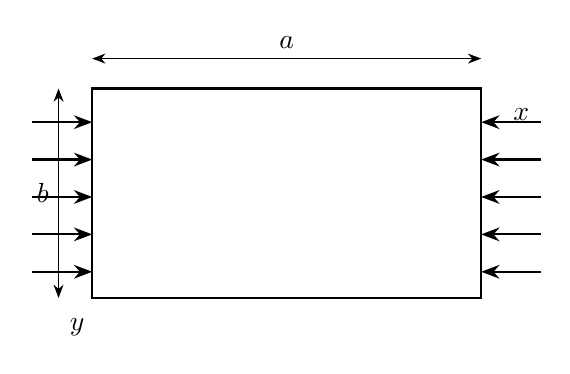
\begin{tikzpicture}[scale=0.95, >=Stealth]
    \draw[line width=0.8pt] (0,0) rectangle (5.2,2.8);
    \draw[<->] (0,3.2) -- (5.2,3.2) node[midway, above] {\(a\)};
    \draw[<->] (-0.45,0) -- (-0.45,2.8) node[midway, left] {\(b\)};
    \foreach \y in {0.35,0.85,1.35,1.85,2.35}
        \draw[->, line width=0.8pt] (-0.8,\y) -- (0,\y);
    \foreach \y in {0.35,0.85,1.35,1.85,2.35}
        \draw[->, line width=0.8pt] (6.0,\y) -- (5.2,\y);
    \node[right] at (5.5,2.45) {\(x\)};
    \node[below] at (-0.2,-0.15) {\(y\)};
\end{tikzpicture}
\caption{單軸壓縮矩形板示意圖：左右邊受 \(x\) 方向面內壓縮。}
\end{figure}

\begin{table}[H]
\centering
\caption{Uniaxial compression, SSSS rectangular plates}
\resizebox{\textwidth}{!}{%
\begin{tabular}{ccccccc}
\toprule
\(a/b\) & nodes & Exact \(k\) & Exact \(\sigma_{cr}\) (psi) & Present \(k\) & Present \(\sigma_{cr}\) (psi) & Error (\%) \\
\midrule
0.2 & 39 & 27.04 & 73317.1 & 352.5498 & 955914.0 & 1203.81 \\
0.3 & 65 & 13.2011 & 35793.9 & 92.5459 & 250931.7 & 601.0459 \\
0.4 & 78 & 8.41 & 22803.1 & 69 & 187088.7 & 720.4518 \\
0.5 & 91 & 6.25 & 16946.4 & 57.7019 & 156454.7 & 823.2301 \\
0.6 & 104 & 5.1378 & 13930.8 & 52.8766 & 143371.2 & 929.1722 \\
0.7 & 117 & 4.5308 & 12284.9 & 49.6183 & 134536.5 & 995.1294 \\
0.8 & 143 & 4.2025 & 11394.8 & 43.1334 & 116953.2 & 926.3748 \\
0.9 & 156 & 4.0446 & 10966.6 & 43.5384 & 118051.3 & 976.4651 \\
1 & 169 & 4 & 10845.7 & 43.6636 & 118390.8 & 991.591 \\
1.1 & 182 & 4.0364 & 10944.4 & 44.5739 & 120859.0 & 1004.29 \\
1.2 & 195 & 4.1344 & 11210.1 & 45.1148 & 122325.6 & 991.1933 \\
1.3 & 221 & 4.2817 & 11609.5 & 43.1664 & 117042.7 & 908.1567 \\
1.4 & 234 & 4.4702 & 12120.6 & 42.3767 & 114901.4 & 847.982 \\
1.41 & 234 & 4.4911 & 12177.3 & 42.5441 & 115355.3 & 847.2997 \\
\bottomrule
\end{tabular}
}
\end{table}

\subsection{純剪矩形板}

此表使用 SSSS 矩形板並施加純剪面內合力。它用來檢查 \(P_{12}\) 進入 \(K^g\) 後，臨界係數對長寬比的變化。材料與厚度設定為 \(E=30\times10^6\) psi、\(\nu=0.3\)、\(k_s=5/6\)、\(h/b=0.01\)，載重為 \(P_{12}=1\)、\(P_{11}=P_{22}=0\)。

\begin{figure}[H]
\centering
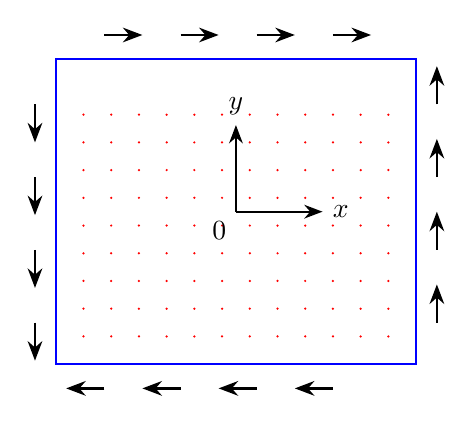
\begin{tikzpicture}[scale=0.88, >=Stealth]
    \draw[blue, line width=0.8pt] (-2.6,-2.2) rectangle (2.6,2.2);
    \foreach \x in {-2.2,-1.8,...,2.2}
        \foreach \y in {-1.8,-1.4,...,1.8}
            \fill[red] (\x,\y) circle (0.018);
    \foreach \x in {-1.9,-0.8,0.3,1.4}
        \draw[->, line width=0.9pt] (\x,2.55) -- ++(0.55,0);
    \foreach \x in {-1.9,-0.8,0.3,1.4}
        \draw[->, line width=0.9pt] (\x,-2.55) -- ++(-0.55,0);
    \foreach \y in {-1.6,-0.55,0.5,1.55}
        \draw[->, line width=0.9pt] (-2.9,\y) -- ++(0,-0.55);
    \foreach \y in {-1.6,-0.55,0.5,1.55}
        \draw[->, line width=0.9pt] (2.9,\y) -- ++(0,0.55);
    \draw[->, line width=0.8pt] (0,0) -- (1.25,0) node[right] {\(x\)};
    \draw[->, line width=0.8pt] (0,0) -- (0,1.25) node[above] {\(y\)};
    \node[below left] at (0,0) {\(0\)};
\end{tikzpicture}
\caption{純剪矩形板示意圖：邊界面內剪力形成 \(P_{12}\) 幾何剛度項。}
\end{figure}

\begin{table}[H]
\centering
\caption{Pure shear, SSSS rectangular plates}
\resizebox{\textwidth}{!}{%
\begin{tabular}{ccccccc}
\toprule
\(a/b\) & nodes & Reference \(k\) & Reference \(\tau_{cr}\) (psi) & Present \(k\) & Present \(\tau_{cr}\) (psi) & Error (\%) \\
\midrule
1 & 169 & 14.71 & 39885.1 & 49.0902 & 133104.6 & 233.7199 \\
1.5 & 247 & 11.5 & 31181.4 & 34.4648 & 93448.9 & 199.6941 \\
2 & 325 & 10.34 & 28036.2 & 29.1745 & 79104.6 & 182.1517 \\
2.5 & 403 & 10.85 & 29419.0 & 26.9588 & 73096.9 & 148.4678 \\
\bottomrule
\end{tabular}
}
\end{table}

\subsection{雙軸壓縮方板}

此表固定 SSSS 方板，改變 \(\gamma=N_y/N_x\)。它用來檢查 \(P_{11}\) 與 \(P_{22}\) 同時作用時的屈曲載重比例。材料與厚度設定為 \(E=30\times10^6\) psi、\(\nu=0.3\)、\(k_s=5/6\)、\(a/b=1\)、\(h/b=0.01\)，載重比例為 \(P_{22}=\gamma P_{11}\)、\(P_{12}=0\)。

\begin{figure}[H]
\centering
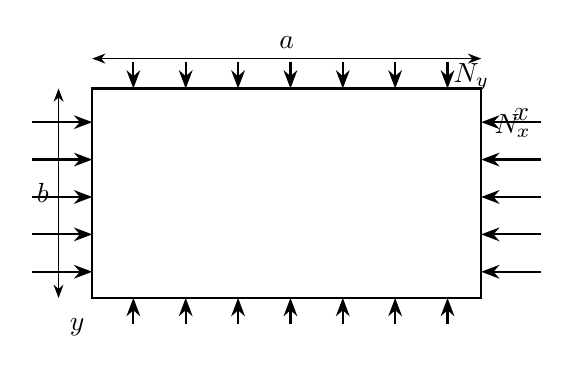
\begin{tikzpicture}[scale=0.95, >=Stealth]
    \draw[line width=0.8pt] (0,0) rectangle (5.2,2.8);
    \draw[<->] (0,3.2) -- (5.2,3.2) node[midway, above] {\(a\)};
    \draw[<->] (-0.45,0) -- (-0.45,2.8) node[midway, left] {\(b\)};
    \foreach \y in {0.35,0.85,1.35,1.85,2.35}
        \draw[->, line width=0.8pt] (-0.8,\y) -- (0,\y);
    \foreach \y in {0.35,0.85,1.35,1.85,2.35}
        \draw[->, line width=0.8pt] (6.0,\y) -- (5.2,\y);
    \foreach \x in {0.55,1.25,1.95,2.65,3.35,4.05,4.75}
        \draw[->, line width=0.8pt] (\x,3.15) -- (\x,2.8);
    \foreach \x in {0.55,1.25,1.95,2.65,3.35,4.05,4.75}
        \draw[->, line width=0.8pt] (\x,-0.35) -- (\x,0);
    \node[right] at (5.5,2.45) {\(x\)};
    \node[below] at (-0.2,-0.15) {\(y\)};
    \node[right] at (5.25,2.3) {\(N_x\)};
    \node[right] at (4.7,2.95) {\(N_y\)};
\end{tikzpicture}
\caption{雙軸壓縮方板示意圖：\(N_y=\gamma N_x\)。}
\end{figure}

\begin{table}[H]
\centering
\caption{Biaxial compression, SSSS square plate}
\resizebox{\textwidth}{!}{%
\begin{tabular}{ccccccc}
\toprule
\(\gamma=N_y/N_x\) & nodes & Exact \(k\) & Exact \(\sigma_{cr}\) (psi) & Present \(k\) & Present \(\sigma_{cr}\) (psi) & Error (\%) \\
\midrule
0 & 169 & 4 & 10845.7 & 43.6636 & 118390.8 & 991.591 \\
0.25 & 169 & 3.2 & 8676.6 & 34.9695 & 94817.3 & 992.7984 \\
0.5 & 169 & 2.6667 & 7230.6 & 29.1466 & 79029.0 & 992.9976 \\
1 & 169 & 2 & 5422.9 & 21.869 & 59296.3 & 993.451 \\
2 & 169 & 1.3333 & 3615.1 & 14.5752 & 39519.6 & 993.1387 \\
4 & 169 & 0.8 & 2169.1 & 8.7407 & 23699.8 & 992.5851 \\
\bottomrule
\end{tabular}
}
\end{table}

\subsection{壓縮與剪力組合方板}

此表固定 SSSS 方板，改變 \(\sigma/\tau\)。它用來檢查壓縮與剪力共同作用時，\(K^g\) 中法向與剪向面內合力的交互影響。材料與厚度設定為 \(E=30\times10^6\) psi、\(\nu=0.3\)、\(k_s=5/6\)、\(a/b=1\)、\(h/b=0.01\)，載重比例由表中的 \(\sigma/\tau\) 指定。

\begin{figure}[H]
\centering
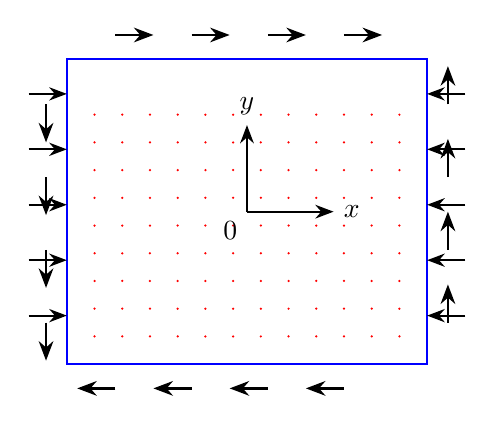
\begin{tikzpicture}[scale=0.88, >=Stealth]
    \draw[blue, line width=0.8pt] (-2.6,-2.2) rectangle (2.6,2.2);
    \foreach \x in {-2.2,-1.8,...,2.2}
        \foreach \y in {-1.8,-1.4,...,1.8}
            \fill[red] (\x,\y) circle (0.018);
    \foreach \y in {-1.5,-0.7,0.1,0.9,1.7}
        \draw[->, line width=0.75pt] (-3.15,\y) -- (-2.6,\y);
    \foreach \y in {-1.5,-0.7,0.1,0.9,1.7}
        \draw[->, line width=0.75pt] (3.15,\y) -- (2.6,\y);
    \foreach \x in {-1.9,-0.8,0.3,1.4}
        \draw[->, line width=0.9pt] (\x,2.55) -- ++(0.55,0);
    \foreach \x in {-1.9,-0.8,0.3,1.4}
        \draw[->, line width=0.9pt] (\x,-2.55) -- ++(-0.55,0);
    \foreach \y in {-1.6,-0.55,0.5,1.55}
        \draw[->, line width=0.9pt] (-2.9,\y) -- ++(0,-0.55);
    \foreach \y in {-1.6,-0.55,0.5,1.55}
        \draw[->, line width=0.9pt] (2.9,\y) -- ++(0,0.55);
    \draw[->, line width=0.8pt] (0,0) -- (1.25,0) node[right] {\(x\)};
    \draw[->, line width=0.8pt] (0,0) -- (0,1.25) node[above] {\(y\)};
    \node[below left] at (0,0) {\(0\)};
\end{tikzpicture}
\caption{壓縮與剪力組合方板示意圖：同時包含 \(P_{11}\) 與 \(P_{12}\)。}
\end{figure}

\begin{table}[H]
\centering
\caption{Combined compression and shear, SSSS square plate}
\resizebox{\textwidth}{!}{%
\begin{tabular}{ccccccccc}
\toprule
\(\sigma/\tau\) & nodes & Reference \(k\) & Reference \(\tau_{cr}\) (psi) & Reference \(\sigma_{cr}\) (psi) & Present \(k\) & Present \(\tau_{cr}\) (psi) & Present \(\sigma_{cr}\) (psi) & Error (\%) \\
\midrule
0 & 169 & 14.71 & 39885.1 & 0.0 & 49.0902 & 133104.6 & 0.0 & 233.7199 \\
0.5 & 169 & 7.09 & 19224.0 & 9612.0 & 33.6204 & 91159.4 & 45579.7 & 374.1952 \\
1 & 169 & 4.5 & 12201.4 & 12201.4 & 25.0189 & 67837.0 & 67837.0 & 455.9759 \\
1.5 & 169 & 3.24 & 8785.0 & 13177.5 & 19.7345 & 53508.7 & 80263.1 & 509.09 \\
2 & 169 & 2.51 & 6805.7 & 13611.4 & 16.2357 & 44022.0 & 88043.9 & 546.8416 \\
\bottomrule
\end{tabular}
}
\end{table}

\section{簡要說明}

Table 1 顯示 Present 值會隨節點密度增加而下降，具備收斂趨勢；Table 2 則顯示目前 Present 與參考方法仍存在明顯尺度差異。補充算例也呈現相同現象，因此後續應優先核對幾何剛度載重尺度、面內合力定義與無因次化轉換。

\end{document}
